\providecommand{\relativeRoot}{../..}
\documentclass[\relativeRoot/main.tex]{subfiles}
\graphicspath{{\subfix{./figures/}}}


\begin{document}

\section{Motivation}
\label{sec:lyprox:motivation}

Publishing and sharing the data of \cref{chap:dataset_usz} with the scientific community is a valuable contribution, since it allows other researchers to test a range of hypotheses. For example, one might be interested in how the involvement of upstream \glspl{lnl} influences the risk of nodal metastases in a given level. Something we have given an answer to in \cref{table:dataset_usz:upstream}. But also theories we did not think of at the time of writing our publications \cite{ludwig_detailed_2021,ludwig_dataset_2021} may be tested by someone who searches the literature for support in favor or against a particular hypothesis.

However, in such a case there are still some hurdles to discovering and taking advantage of freely available data: The researcher -- who we assume to have already conceived their hypothesis -- needs to understand what is reported in the dataset, what format it is provided in and how to implement a test using the found information. Our data is provided as a \gls{csv} table, meaning it can be opened in a spreadsheet program like Microsoft Excel. This would allow the user to create e.g. pivot tables and derived variables from observed ones, after they have made themselves familiar with the description and meaning of all the provided columns.

Taking these steps is not particularly difficult, and a determined scientist may be able to accomplish that in a matter of hours. However, if a researcher came up with a quick idea, not yet fully developed into a hypothesis, the outlined procedure could -- in their eyes -- very well not be worth the potential insight. Consequently, an interesting idea and a valuable cohort of patients might be left unexplored. Even more so in case of someone who did not even come up with a research question yet our data may be able to answer.

Figures and tables, like \cref{fig:dataset_usz:statistics} and \cref{table:dataset_usz:prevalence} that allow a reader of our work to quickly and visually understand our data address these issues to some extent. They create an understanding of what is reported in the data and answer common questions about it. But it is not feasible to provide plots and tables on all aspects of a dataset within a publication.

\subsection*{Prototype}
\label{subsec:lyprox:motivation:prototype}

This is why we thought of providing a dashboard, allowing a user to create the visualizations and numbers themselves according to their interest w.r.t. the underlying data. The first implementation that provided such a dashboard was a Python-based \gls{gui} developed by Bertrand Pouymayou for the use on local hardware (e.g. a laptop). It could display the prevalence of involvement for all \glspl{lnl} while the patients could be stratified by a number of variables that were recorded (e.g. smoking status). Moreover, one could explore how frequently certain levels were involved together or on their own. With this \gls{gui} it is possible, for example, to investigate the frequency of involvement in a certain level without metastases in an upstream \glspl{lnl}. A screenshot of this first prototype is shown in \cref{fig:lyprox:pouymayou_gui}.

\begin{figure}
    \centering
    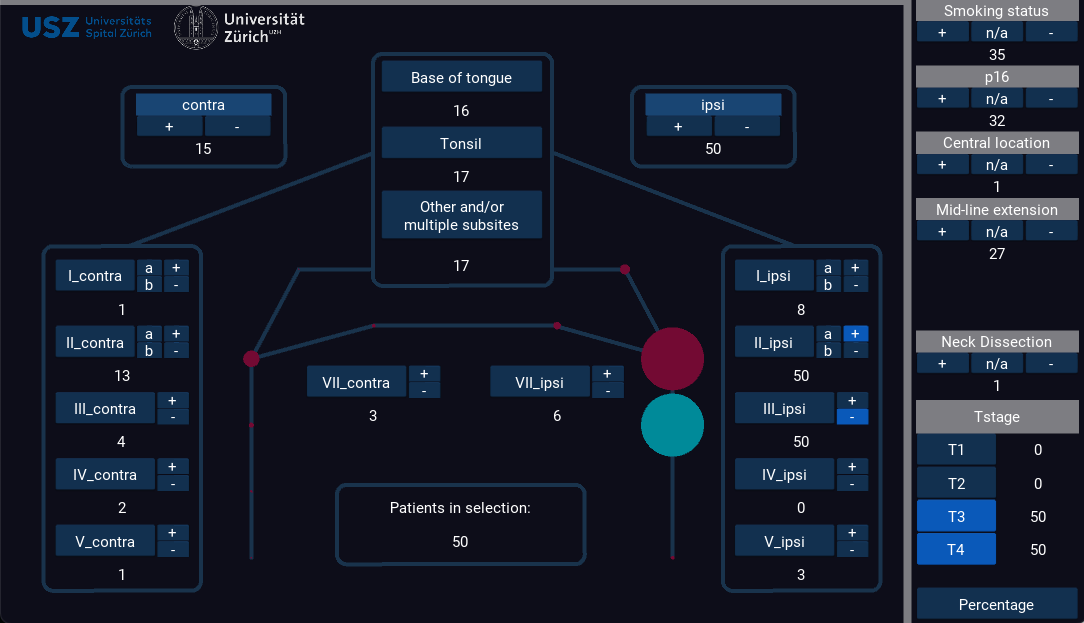
\includegraphics[width=1.0\textwidth]{figures/pouymayou_gui.png}
    \caption[
        Prototype of a GUI to explore patterns of lymphatic progression
    ]{
        Python-based \gls{gui} as developed by Bertrand Pouymayou to interactively explore our dataset containing patterns of lymphatic progression. The sidebar on the right allows stratification w.r.t. patient and tumor information, e.g. smoking status, lateralization of the primary tumor or T-category. In the center, patients can be selected based in primary tumor subsites. The boxes named e.g. \texttt{III\_ipsi} allowed to (de)select patients with metastases in the respective \gls{lnl}.
    }
    \label{fig:lyprox:pouymayou_gui}
\end{figure}

The prototype already allowed us to quickly check correlation and patterns without having to manually go through large tables. Distributing this version of the \gls{gui} such that anyone could obtain a copy of it, install and subsequently run it, however, would have faced difficulties. Making \acrlongpl{gui} platform-independent is usually very error-prone and requires care w.r.t. to the installation and set up process. Moreover, not all potential users are necessarily familiar with the tools required. Hence, we decided to provide the interface such that we set up and control the environment it runs in.

\subsection*{Online Interface}
\label{subsec:lyprox:motivation:online}

Arguably the most broadly accessible and most easily usable type of user interface comes in the form of interactive web pages. Consisting of \faIcon{html5}~\acrshort{html} documents styled using \faIcon{css3-alt}~\acrshort{css}, web pages require nothing but a modern web browser, of which a large number is available on all kinds of platforms and hardware, and an internet connection. So, in order to make our visualization tool as easily accessible as possible, we decided to develop a web-based \gls{gui}.

Because of how ubiquitous and important web content has become, the demand for efficient and versatile tools to develop that content is very high. Consequently, there exists a plethora of frameworks and technologies we needed to choose from before starting to build our \gls{gui}. The first choice however, is which type of web page we wanted to serve, as they can broadly be grouped into two types:

\begin{itemize}
    \item \textbf{Static:} For these kinds of web pages, the server sends the content to the client or user as it is stored. This means that no logic is executed by the server and different users always receive the same content. However, the resulting web page, as it is rendered on the client's side, may still be interactive, since entire programs can be embedded into it and run inside the user's browser.
    \item \textbf{Dynamic:} In this case, the server reacts \emph{dynamically} to the request sent to it by the user. The request is processed based on the programmed logic and a corresponding response is rendered and sent back.
\end{itemize}

Of course, hybrid approaches are also possible and in fact very common, as client-side executed scripts can almost always be added to a dynamically served web page. 

We decided to build a \emph{dynamic} site for two main reasons: 
\begin{enumerate*}[label={(\arabic*)}]
    \item If it were static, the underlying data would need to be sent alongside the layout, design and logic of the interface. And as the data may at some point include thousands of patients, the initial loading times could become very long. Processing the data on the server side and only sending the computed results (e.g. a prevalence of lymphatic involvement) remains feasible, even as the database grows.
    \item Implementing logic on the client side usually requires it to be programmed in the \faIcon{js-square}~JavaScript language, which we are not very proficient with. In the backend on the server, however, the logic that compiles and renders the web page in the dynamic case can be implemented in a number of programming languages. This means we were able to choose the development framework based on our skill set.
\end{enumerate*}

At the time of beginning the development for the \gls{gui}, we had already implemented the probabilistic model that we will introduce in \cref{chap:unilateral} in the programming language \faIcon{python}~Python. Hence, we decided to use a web framework also implemented in that language, since it matched our skills and may allow us to add that model's library directly into the \gls{gui}'s logic.

Even when one has settled on a dynamic website that serves content using a backend written in \faIcon{python}~Python, there are still numerous frameworks to choose from, e.g. \href{https://flask.palletsprojects.com/en/2.2.x/}{Flask}, \href{https://plotly.com/dash/}{Dash} or \href{http://bottlepy.org/docs/dev/}{Bottle}. However, we decided to go with \href{https://www.djangoproject.com/}{Django} \cite{noauthor_django_2022}, as it is one of the most popular ones and comes with numerous features -- especially related to security and authorization -- already built-in. It makes heavy use of the \gls{oop} paradigm, especially for its database models, which -- as we will see -- made it easy for us to represent e.g. a patient within Django.

\end{document}
